\subsection{Latency}
\label{sec:ip-timing}

% Data Occurrence analysis
Feed latency measures how quickly a feed reports new threat indicators. The
sooner a feed can report potential threats, the more valuable it is for
consumers. The absolute latency of an indicator in a feed is the time from
the beginning of the corresponding event until when the indicator shows up in
the feed. However, it is difficult to know the actual time when an event begins
from the threat intelligence data. Instead, we measure the \textit{relative
latency}, which is the delay of an indicator in one feed to be the time between
its appearance in that feed and the first seen among all the feeds.

\begin{figure}[t!]
\centering
\subfloat[Latency distribution in scan feeds]{
	\label{fig:scan_firstseen}
	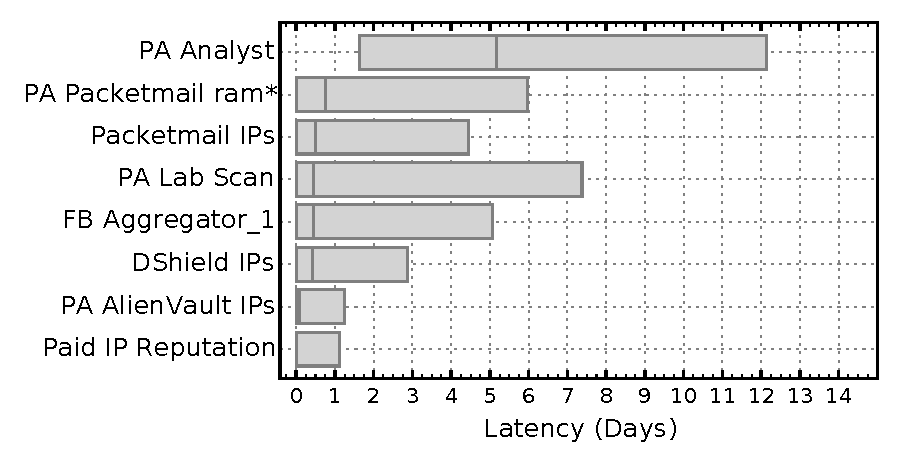
\includegraphics[width=0.8\textwidth]{data_character/images/scan_latency_new.pdf}}

\subfloat[Latency distribution in brute-force feeds]{
	\label{fig:brute_firstseen}
	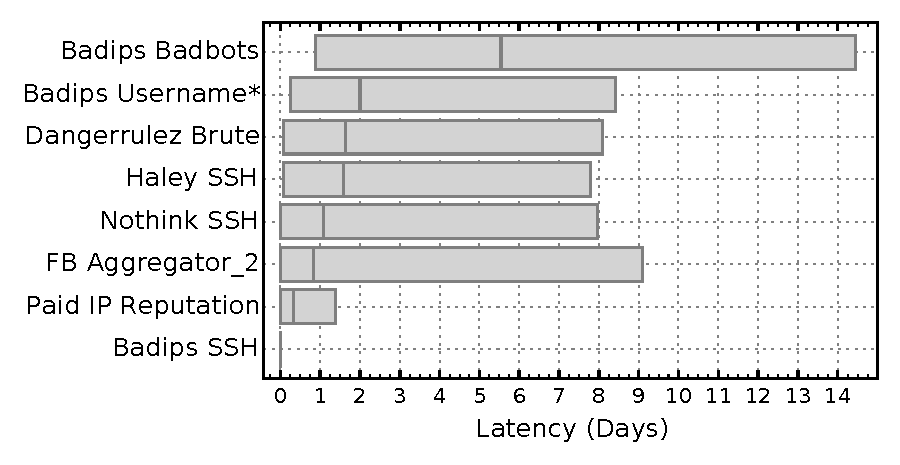
\includegraphics[width=0.8\textwidth]{data_character/images/brute_latency_new.pdf}}

\caption{Distribution of indicators' latency in scan and brute-force feeds.}
\label{fig:firstseen}
\end{figure}


Relative latency can only be calculated for
indicators that occur in at least two feeds. As discussed in
Section~\ref{sec:ip-unique}, the number of common indicators in the botnet, malware, exploit and spam feeds is very low (fewer than 3\% of elements occur in more than one feed). Relative latency calculated for these feeds is less meaningful. For this analysis, therefore, we focus on scan and brute-force feeds.

Another issue is the time sensitivity of IP threats. An event that originated from
an IP address, like scanning activity or a brute-force attack, will not last
forever. If one scan feed reports an IP address today and another feed reports
the same IP three months later, it would make little sense to consider them as one
scanning event and label the second occurrence as being three months late.
Unfortunately, there is no easy way we can clearly distinguish events from each
other. Here we use a one-month window to restrict an event, assuming that the same
attack from one source will not last for more than 30 days; although arbitrary, it provides a reasonably conservative threshold, and experimenting with other thresholds produced similar overall results. More specifically, we calculate relative latency by tracking the
first occurrence of IPs in all feeds in a category, then recording the latency of the
following occurrences while excluding ones that occur after 30 days. By just
using the first appearance of each IP as the base, we avoid the uncertainty caused by
multiple occurrence of indicators and different valid periods used among feeds.

%We also used other time windows for the latency calculation and the results are very similar.

Figures~\ref{fig:scan_firstseen} and~\ref{fig:brute_firstseen} show the relative
latency distribution among feeds in the scan and brute-force categories, in hours. Each box shows the latency distribution of shared IPs in the feed calculated in hours
from 25 percentile to 75 percentile, with the middle line indicating the median.
(``Badips Username*'' here is the abbreviation for feed name Badips
Username Notfound; ``PA Packetmail Ram*'' for PA Packetmail Ramnode)
We focus on just those feeds that have
over 10\% of their data shared with others to ensure the analysis can represent the latency
distribution of the overall feed. There is one feed in each category ({\feedTSSnort}
in scan and {\feedTSBrute} in brute-force) that is excluded from the figure.

\finding\
From the distribution boxes we can see that {\feedetiprep} in scan and {\feedbadipssh}
in brute-force are the fastest feeds in their category, as they have the lowest median
and 75th percentile latencies. On the other hand, {\feedTSAnalyst} in scan and
{\feedbadipbot} in brute-force are the slowest feeds. Figure~\ref{fig:scan_firstseen}
shows that all scan feeds except one have their 25th percentile latency equal to 0, indicating
these feeds, across different sizes, all reported a significant portion of their shared
data first. A similar case also happens in the brute-force category.

%This means that feeds can scan feeds, no matter fast or slow,

One may reasonably ask whether large feeds report data sooner than small feeds.
The result shows that this is not always the case. {\feedFBBasecamp} is the second smallest
feed in our scan category, yet it is no slower than several other feeds which have over 10 times of its daily rate.
{\feedbadipbot}, on the other hand, has the second largest rate in brute-force
category, but it is slower than all the other feeds in the brute-force category. Feeds that are small in volume can still report a lot of their data first.

% This shows that when choosing a feed, we cannot assume its latency by just looking at its volume.

Another factor that could affect latency is whether feeds copy data from each other. For example, 93\% of {\feeddangerrule} also appears in {\feedbadipssh}. If this is the case, we expect {\feeddangerrule} will be faster than {\feedbadipssh} on
reporting their shared data. However, we compared the relative latency between just two feeds and found {\feedbadipssh} reported 88\% of their shared indicators first.
We further conducted this pairwise latency comparison between all feeds in scan, brute-force
and malware (since {\feedetiprep} shares non-trivial amount of data with a
few small feeds in the malware category), and did not see a clear latency advantage between
any two feeds. Note that this observation does \emph{not} prove there is no data
copying, since the shared data between two feeds might partially come from copying and partially from the feeds' own data collection. Furthermore, our latency analysis is at a one-hour granularity.
% We did not find the evidence in latency to prove that there is indeed data copying.
